\documentclass{tufte-handout}\usepackage[]{graphicx}\usepackage[]{color}
%% maxwidth is the original width if it is less than linewidth
%% otherwise use linewidth (to make sure the graphics do not exceed the margin)
\makeatletter
\def\maxwidth{ %
  \ifdim\Gin@nat@width>\linewidth
    \linewidth
  \else
    \Gin@nat@width
  \fi
}
\makeatother

\definecolor{fgcolor}{rgb}{0.345, 0.345, 0.345}
\newcommand{\hlnum}[1]{\textcolor[rgb]{0.686,0.059,0.569}{#1}}%
\newcommand{\hlstr}[1]{\textcolor[rgb]{0.192,0.494,0.8}{#1}}%
\newcommand{\hlcom}[1]{\textcolor[rgb]{0.678,0.584,0.686}{\textit{#1}}}%
\newcommand{\hlopt}[1]{\textcolor[rgb]{0,0,0}{#1}}%
\newcommand{\hlstd}[1]{\textcolor[rgb]{0.345,0.345,0.345}{#1}}%
\newcommand{\hlkwa}[1]{\textcolor[rgb]{0.161,0.373,0.58}{\textbf{#1}}}%
\newcommand{\hlkwb}[1]{\textcolor[rgb]{0.69,0.353,0.396}{#1}}%
\newcommand{\hlkwc}[1]{\textcolor[rgb]{0.333,0.667,0.333}{#1}}%
\newcommand{\hlkwd}[1]{\textcolor[rgb]{0.737,0.353,0.396}{\textbf{#1}}}%

\usepackage{framed}
\makeatletter
\newenvironment{kframe}{%
 \def\at@end@of@kframe{}%
 \ifinner\ifhmode%
  \def\at@end@of@kframe{\end{minipage}}%
  \begin{minipage}{\columnwidth}%
 \fi\fi%
 \def\FrameCommand##1{\hskip\@totalleftmargin \hskip-\fboxsep
 \colorbox{shadecolor}{##1}\hskip-\fboxsep
     % There is no \\@totalrightmargin, so:
     \hskip-\linewidth \hskip-\@totalleftmargin \hskip\columnwidth}%
 \MakeFramed {\advance\hsize-\width
   \@totalleftmargin\z@ \linewidth\hsize
   \@setminipage}}%
 {\par\unskip\endMakeFramed%
 \at@end@of@kframe}
\makeatother

\definecolor{shadecolor}{rgb}{.97, .97, .97}
\definecolor{messagecolor}{rgb}{0, 0, 0}
\definecolor{warningcolor}{rgb}{1, 0, 1}
\definecolor{errorcolor}{rgb}{1, 0, 0}
\newenvironment{knitrout}{}{} % an empty environment to be redefined in TeX

\usepackage{alltt}

%\documentclass{article}
\usepackage{graphicx}
%\setkeys{Gin}{width=\linewidth,totalheight=\textheight,keepaspectratio}
% Prints a trailing space in a smart way.
\usepackage{xspace}
\usepackage{hyperref}
\usepackage{amsmath}
\newcommand{\tthdump}[1]{#1}
\usepackage{makeidx}
\usepackage{tabularx}

%\makeindex

\begin{knitrout}
\definecolor{shadecolor}{rgb}{0.969, 0.969, 0.969}\color{fgcolor}\begin{kframe}


{\ttfamily\noindent\color{warningcolor}{\#\# Warning: No security definition has been found for the request}}\begin{verbatim}
## failed to load HTTP resource
\end{verbatim}


{\ttfamily\noindent\bfseries\color{errorcolor}{\#\# Error: 1: failed to load HTTP resource}}\end{kframe}
\end{knitrout}


\title{Buy On Gap trading report - S\&P 500}

\date{ 23 Dec 2013 }

\IfFileExists{upquote.sty}{\usepackage{upquote}}{}


\begin{document}
\maketitle

%\SweaveOpts{concordance=TRUE}
%\setkeys{Gin}{width=1.1\marginparwidth} %% Sweave

\section{Trade execution}
\subsection{Order executed}

% latex table generated in R 3.0.2 by xtable 1.7-1 package
% Tue Dec 24 05:10:12 2013
\begin{table}[ht]
\centering
\begin{tabular}{llrrrrrrr|r}
  \hline
 & Symbol & B.AvgPrc & B.Qty & S.AvgPrc & S.Qty & Profit & Comm. & Return \% & Closing Price \\ 
  \hline
1 & MU & 21.39 & 4179 & 21.49 & 4179 & 374.55 & 43.35 & 0.42 & 21.50 \\ 
   \hline
\end{tabular}
\end{table}



\subsection{Stock Portfolio}
% latex table generated in R 3.0.2 by xtable 1.7-1 package
% Tue Dec 24 05:10:12 2013
\begin{table}[ht]
\centering
\begin{tabular}{llrrr}
  \hline
 & Symbol & Quantity & Closing price & Market price \\ 
  \hline
1 & ***NO-ASSET*** &  &  &  \\ 
   \hline
\end{tabular}
\end{table}



\section{Trading Matrix}


% latex table generated in R 3.0.2 by xtable 1.7-1 package
% Tue Dec 24 05:10:12 2013
\begin{table}[ht]
\begin{tabular}{lr}
   \hline
Portofolio Amount: & 89859.66 \\ 
  Asset Amount: & 0.00 \\ 
  Bought Amount: & 89388.81 \\ 
  Sold   Amount: & 89806.71 \\ 
  Commission   : & 43.35 \\ 
  P/L incl Comm: & 374.55 \\ 
  Ret incl Comm \%: & 0.42 \\ 
  S\&P 500 Ret \%: & 0.53 \\ 
   \hline
\end{tabular}
\caption{The commissions and daily returns are calculated based on the closed position.
The open position is present in the portofolio and assume closing on the next open market.
Portofolio amount is the open order with today closing price.} 
\end{table}



% \section{Trade Slippage}
% 
% <<slippage, echo = FALSE , results='asis'>>=
% 
% colnames(slippage) <- c('Symbol','Open Slippage %', 'Close Slippage %');
% print(xtable(slippage),floating=FALSE,);
% @


\title{Buy On Gap trading report - S\&P 600}
\maketitle

\section{Trade execution}
\subsection{Order executed}


% latex table generated in R 3.0.2 by xtable 1.7-1 package
% Tue Dec 24 05:10:12 2013
\begin{table}[ht]
\centering
\begin{tabular}{llrrrrrrr|r}
  \hline
 & Symbol & B.AvgPrc & B.Qty & S.AvgPrc & S.Qty & Profit & Comm. & Return \% & Closing Price \\ 
  \hline
\hline
\end{tabular}
\end{table}



\subsection{Stock Portfolio}
No stock hold in the portfolio at the end of the day.


\section{Trading Matrix}

% latex table generated in R 3.0.2 by xtable 1.7-1 package
% Tue Dec 24 05:10:12 2013
\begin{table}[ht]
\begin{tabular}{lr}
   \hline
Portofolio Amount: &  \\ 
  Asset Amount: &  \\ 
  Bought Amount: &  \\ 
  Sold   Amount: &  \\ 
  Commission   : &  \\ 
  P/L incl Comm: &  \\ 
  Ret incl Comm \%: &  \\ 
  S\&P 600 Ret \%: &  \\ 
   \hline
\end{tabular}
\caption{The commissions and daily returns are calculated based on the closed position.
The open position is present in the portofolio and assume closing on the next open market.
Portofolio amount is the open order with today closing price.} 
\end{table}



% \section{Trade Slippage}
% 
% <<slippage_sp600, echo = FALSE , results='asis'>>=
% 
% colnames(slippage) <- c('Symbol','Open Slippage %', 'Close Slippage %');
% print(xtable(slippage),floating=FALSE,);
% @

\newpage
\section{News}

%\begin{margintable}

% latex table generated in R 3.0.2 by xtable 1.7-1 package
% Tue Dec 24 05:10:12 2013
\begin{tabularx}{\textwidth}{rX}
  \hline
 & MU \\ 
  \hline
1 &  Micron Technology Appoints Rajan Rajgopal as Vice President of Quality  -  MarketWatch Decisions Made Micron Technology, Inc. (NASDAQ:MU) An Attractive Buy  -  US Trade Media \\ 
  2 &  Micron Technology, Inc. (NASDAQ:MU) could benefit from the DRAM Wuxi output constraints that could drag into February versus prior expectations of late December - January.  \\ 
  3 &  Micron Technology, Inc. : Rambus and Micron Sign License Agreement  -  4-traders (press release) Micron Technology, Inc. (NASDAQ:MU) Inks Agreement With Rambus Inc ...  -  USTrade Voice \\ 
  4 &  While Fools should generally take the opinion of Wall Street with a grain of salt, it's not a bad idea to take a closer look at particularly stock-shaking upgrades and downgrades  \\ 
  5 &  As of late, it has definitely been a great time to be an investor in Micron Technology, Inc. (MU). The stock has moved higher by 20.3\% in the past month, while it is also above its 20 Day SMA too.  \\ 
  6 &  Tomahawk, WI 12/17/2013 (BasicsMedia) - Micron Technology, Inc. (NASDAQ:MU) is the global No. 5 semiconductor company.  \\ 
  7 &  Boston, MA 12/19/2013 (wallstreetpr) - Micron Technology, Inc. (NASDAQ:MU)'s shares fell by almost 5\% to close at \$21.81 on rumors that Hynix, one of the competitors would be expanding its capacity.  \\ 
  8 &  Micron Technology (MU) dropped lower to \$22.77 versus \$23.08 last week. The leading provider of semiconductor solutions was unable to escape the heightened anxiety of investors as they anticipate the results of the Federal Reserve policy meeting which ...  \\ 
  9 &  A roundup of tech ratings changes. Micron (MU -3\%) has been cut to Underperform by BofA/Merrill. Shares fell last week in response to a Bloomberg report stating SK Hynix plans to build a new DRAM fab.  \\ 
  10 &  New York, December 23, 2013 / Accesswire / - Market Buzz Report, which provides live alerts on penny stocks, issues critical stocks analysis for Apple Inc.(NASDAQ:AAPL), Micron Technology, Inc. (NASDAQ:MU), BlackBerry Ltd (NASDAQ:BBRY), Nokia ...  \\ 
   \hline
\end{tabularx}


%\end{margintable}

\newpage
\section{Individual contract}
\begin{fullwidth}
\begin{knitrout}
\definecolor{shadecolor}{rgb}{0.969, 0.969, 0.969}\color{fgcolor}\begin{kframe}


{\ttfamily\noindent\bfseries\color{errorcolor}{\#\# Error: chartSeries requires an xtsible object}}\end{kframe}
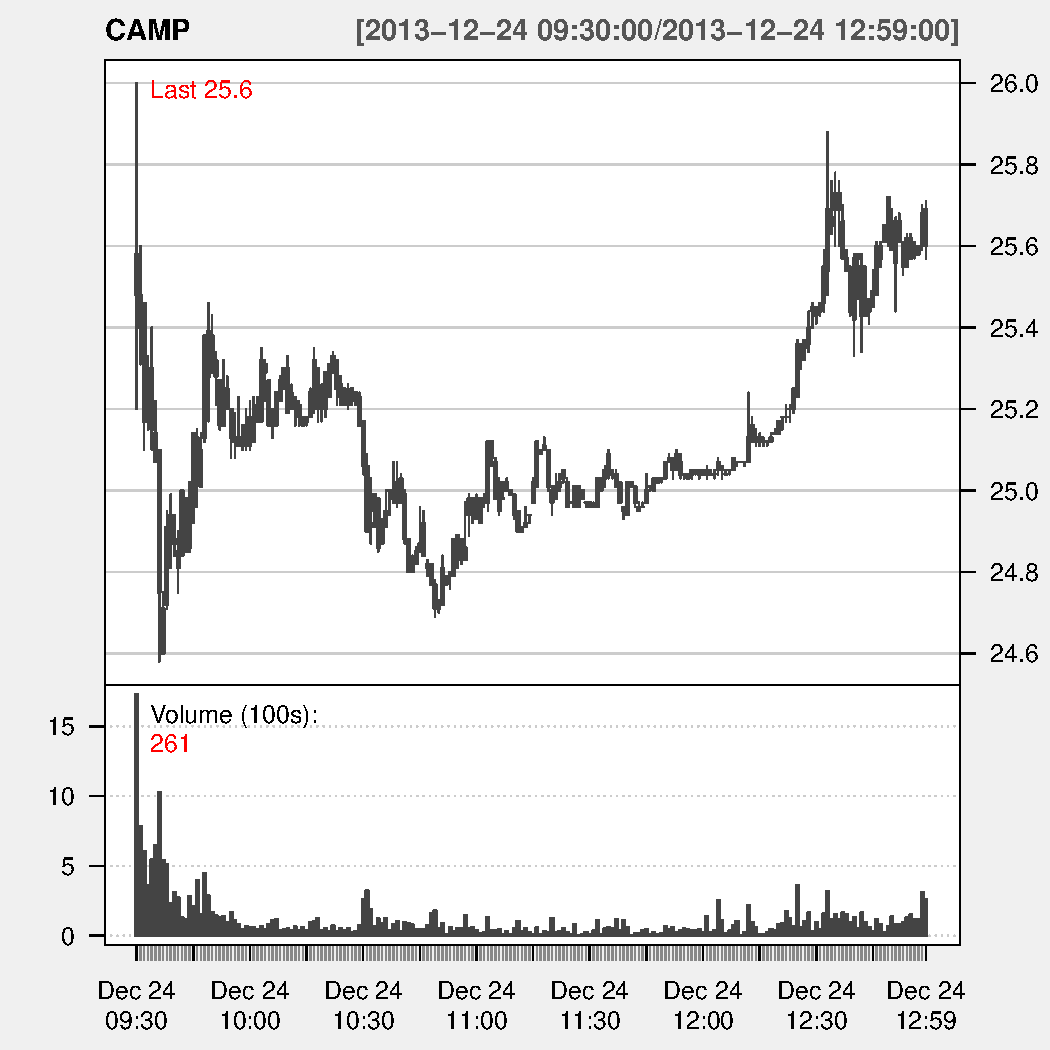
\includegraphics[width=\maxwidth]{/home/jhleong/dev/R/buy_on_gap/BuyOnGap_report/figure/price_chart} 

\end{knitrout}


\end{fullwidth}
\end{document}
